\documentclass[12pt,a4paper]{article} 

\usepackage[utf8]{inputenc}
\usepackage[T1]{fontenc}
\usepackage{amsmath, amssymb, amsthm}
\usepackage[dvipsnames]{xcolor}
\usepackage{geometry}
\usepackage{booktabs}
\usepackage{hyperref}
\usepackage{parskip}
\usepackage{tikz}
\usetikzlibrary{arrows.meta, calc, decorations.markings}

\geometry{margin=2.5cm}
\hypersetup{colorlinks=true, linkcolor=blue!60!black,
            citecolor=blue!60!black, urlcolor=blue!60!black}

\newtheorem{remark}{Observacion}
\newtheorem{definition}{Definicion}

\title{\textbf{Integrales de Linea}\\[0.5em]
\large Trabajo en un Campo de Fuerza, Parametrizacion y Elementos\\[0.3em]
\normalsize Notas para un Curso de Maestria en Boundary Element Method}
\author{W.F. Florez\\
\small Wessex Institute of Technology}
\date{}

\begin{document}

\maketitle
\tableofcontents
\newpage

% ─────────────────────────────────────────────────────────────
\section{Motivacion Fisica: Trabajo en un Campo de Fuerza}
% ─────────────────────────────────────────────────────────────

\subsection{Definicion de Trabajo}

Consideremos una particula que se mueve a lo largo de una curva $\mathcal{C}$
en el plano, sometida a un campo de fuerzas vectorial:

\begin{equation}
    \mathbf{F}(x,y) = \begin{pmatrix} P(x,y) \\ Q(x,y) \end{pmatrix}
\end{equation}

El trabajo elemental realizado por $\mathbf{F}$ al desplazar la particula
un tramo infinitesimal $d\mathbf{r} = (dx,\, dy)^T$ es:

\begin{equation}
    dW = \mathbf{F} \cdot d\mathbf{r} = P\,dx + Q\,dy
\end{equation}

El trabajo total a lo largo de $\mathcal{C}$ es la \textbf{integral de linea}:

\begin{equation}
\boxed{
    W = \int_\mathcal{C} \mathbf{F} \cdot d\mathbf{r}
      = \int_\mathcal{C} P\,dx + Q\,dy
}
\label{eq:trabajo}
\end{equation}

\begin{definition}
La integral de linea de un campo vectorial $\mathbf{F}$ a lo largo de
una curva orientada $\mathcal{C}$ es la integral \eqref{eq:trabajo}.
La orientacion de $\mathcal{C}$ importa: invertir el sentido de recorrido
cambia el signo de $W$.
\end{definition}

\subsection{Por que no Puede Evaluarse Directamente}

La integral \eqref{eq:trabajo} no es una integral ordinaria sobre $x$ o
sobre $y$: las variables $x$ e $y$ estan ligadas por la geometria de
$\mathcal{C}$ y no pueden variar independientemente.

Para ver esto con un ejemplo concreto, consideremos el semicirculo superior
de radio $R$, recorrido de $(R,0)$ a $(-R,0)$. Para cada valor de
$x \in [-R, R]$ existe exactamente un punto sobre la curva, pero $dy$ no
esta determinado solo por $dx$: depende de la direccion tangente en ese
punto, que cambia continuamente a lo largo del arco.

Intentar escribir $\int_{R}^{-R} P\,dx$ sin especificar la curva es
ambiguo porque el mismo par de extremos puede conectarse por infinitas
trayectorias distintas, cada una dando un valor diferente de $W$ en
general.

\begin{remark}
Solo cuando el campo es \textbf{conservativo}, es decir
$\mathbf{F} = \nabla\varphi$ para algun potencial $\varphi$, el trabajo
es independiente de la trayectoria y depende solo de los extremos. En
ese caso $W = \varphi(B) - \varphi(A)$, que es el analogo exacto de la
formula $I = \phi(b) - \phi(a)$ que derivamos en la cuadratura DR-1D.
\end{remark}

% ─────────────────────────────────────────────────────────────
\section{La Parametrizacion como Solucion}
% ─────────────────────────────────────────────────────────────

\subsection{Reduccion a una Integral Ordinaria}

Se introduce un parametro $t \in [a,b]$ que recorre la curva de forma
monótona:

\begin{equation}
    \mathbf{r}(t) = \begin{pmatrix} x(t) \\ y(t) \end{pmatrix},
    \qquad t \in [a,b]
    \label{eq:param}
\end{equation}

Entonces $dx = x'(t)\,dt$ y $dy = y'(t)\,dt$, y la integral de linea se
convierte en una integral ordinaria sobre $t$:

\begin{equation}
\boxed{
    W = \int_a^b \Bigl[ P(x(t),\,y(t))\,x'(t)
                      + Q(x(t),\,y(t))\,y'(t) \Bigr]\, dt
}
\label{eq:param_integral}
\end{equation}

Esta integral puede evaluarse con cualquier metodo de cuadratura estandar
porque el integrando es ahora una funcion escalar de una sola variable $t$.

\subsection{Ejemplo Analitico: Campo Rotacional sobre el Semicirculo}

\textbf{Campo:} $\mathbf{F}(x,y) = (-y,\, x)$, es decir $P = -y$, $Q = x$.

\textbf{Curva:} semicirculo superior de radio $R$, de $(R,0)$ a $(-R,0)$:

\begin{equation}
    \mathbf{r}(t) = \begin{pmatrix} R\cos t \\ R\sin t \end{pmatrix},
    \qquad t \in [0, \pi]
\end{equation}

\textbf{Derivadas:}

\begin{equation}
    x'(t) = -R\sin t, \qquad y'(t) = R\cos t
\end{equation}

\textbf{Integrando:}

\begin{align}
    P\,x' + Q\,y'
    &= (-R\sin t)(-R\sin t) + (R\cos t)(R\cos t) \notag \\
    &= R^2\sin^2 t + R^2\cos^2 t = R^2
\end{align}

\textbf{Integral:}

\begin{equation}
    W = \int_0^\pi R^2\, dt = \pi R^2
    \label{eq:sol_analitica}
\end{equation}

El resultado $W = \pi R^2$ tiene una interpretacion geometrica directa:
es el area del semicirculo de radio $R$. Esta coincidencia no es casual ---
el campo $\mathbf{F} = (-y, x)$ tiene rotacional $\nabla\times\mathbf{F} = 2$,
y por el Teorema de Green el trabajo sobre una curva cerrada seria el doble
del area encerrada.

\begin{figure}[h]
\centering
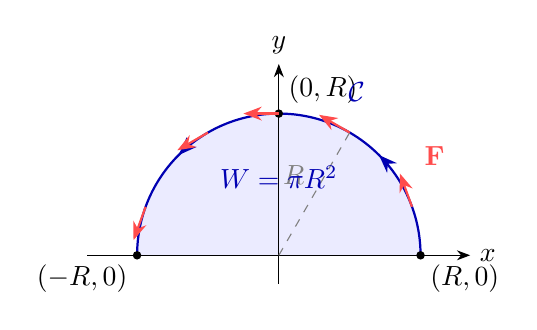
\begin{tikzpicture}[scale=1.8,
    >={Stealth}]

    % Relleno del semicirculo
    \fill[blue!8] (1,0) arc[start angle=0, end angle=180, radius=1]
                  -- cycle;

    % Eje x
    \draw[->] (-1.35,0) -- (1.35,0) node[right] {$x$};
    \draw[->] (0,-0.2)  -- (0,1.35)  node[above] {$y$};

    % Semicirculo con flecha de orientacion
    \draw[blue!70!black, thick,
        postaction={decorate,
            decoration={markings,
                mark=at position 0.25 with {\arrow{Stealth}},
                mark=at position 0.75 with {\arrow{Stealth}}}}]
        (1,0) arc[start angle=0, end angle=180, radius=1];

    % Extremos
    \fill[black] ( 1,0) circle (0.03) node[below right] {$(R,0)$};
    \fill[black] (-1,0) circle (0.03) node[below left]  {$(-R,0)$};
    \fill[black] ( 0,1) circle (0.03) node[above right] {$(0,R)$};

    % Radio R
    \draw[gray, dashed] (0,0) -- ({cos(60)},{sin(60)})
        node[midway, above left] {$R$};

    % Vectores del campo en varios puntos
    \foreach \ang/\sc in {20/0.25, 60/0.25, 90/0.25, 120/0.25, 160/0.25}{
        \pgfmathsetmacro{\xp}{cos(\ang)}
        \pgfmathsetmacro{\yp}{sin(\ang)}
        \draw[->, red!70, thick]
            (\xp,\yp) --
            ({\xp + \sc*(-\yp)},{\yp + \sc*\xp});
    }

    % Etiquetas
    \node[blue!70!black] at (0.0, 0.55) {$W = \pi R^2$};
    \node[red!70]        at (1.1, 0.7)  {$\mathbf{F}$};
    \node[blue!70!black] at (0.55,1.15) {$\mathcal{C}$};
\end{tikzpicture}
\caption{Campo rotacional $\mathbf{F} = (-y, x)$ (flechas rojas) sobre el
semicirculo superior de radio $R$ (azul). El trabajo total $W = \pi R^2$
coincide con el area del semicirculo.}
\end{figure}

% ─────────────────────────────────────────────────────────────
\section{Discretizacion en Elementos}
% ─────────────────────────────────────────────────────────────

\subsection{Necesidad de Discretizar}

Para curvas generales, la integral \eqref{eq:param_integral} rara vez
tiene solucion analitica. La evaluacion numerica requiere dividir
$\mathcal{C}$ en segmentos simples sobre los cuales la cuadratura de
Gauss sea eficiente. Cada uno de estos segmentos es un \textbf{elemento}.

\subsection{Division en $N_e$ Elementos}

Se divide el intervalo parametrico $[a,b]$ en $N_e$ subintervalos:

\begin{equation}
    a = t_0 < t_1 < t_2 < \cdots < t_{N_e} = b
\end{equation}

cada uno correspondiendo a un elemento $\mathcal{C}_k$, $k=1,\ldots,N_e$:

\begin{equation}
    \mathcal{C}_k: \quad t \in [t_{k-1},\, t_k]
\end{equation}

La integral total se descompone:

\begin{equation}
    W = \sum_{k=1}^{N_e} \int_{t_{k-1}}^{t_k}
    \Bigl[ P\,x' + Q\,y' \Bigr]\, dt
\end{equation}

Sobre cada elemento se introduce un parametro local $\xi \in [-1,1]$
(el intervalo estandar de Gauss-Legendre) mediante:

\begin{equation}
    t = \frac{t_{k-1}+t_k}{2} + \frac{t_k - t_{k-1}}{2}\,\xi
\end{equation}

\subsection{Tres Tipos de Elementos}

La diferencia entre los tipos de elementos reside en como se aproxima la
geometria $\mathbf{r}(\xi)$ dentro de cada elemento.

\subsubsection{Elemento Constante}

La curva se aproxima por un segmento recto y el integrando se evalua
unicamente en el punto medio del elemento. Es el mas simple pero el menos
preciso geometricamente.

\subsubsection{Elemento Lineal}

La curva se aproxima por el segmento recto entre los dos nodos extremos,
y el integrando se interpola linealmente. Es el caso que desarrollaremos
en detalle.

\subsubsection{Elemento Cuadratico}

Se usan tres nodos por elemento (dos extremos y uno interior) y tanto la
geometria como el integrando se aproximan por un polinomio de grado 2.
Puede capturar curvatura local y es el estandar en BEM moderno.

\subsection{Elemento Lineal: Desarrollo Completo}

Sobre el elemento $\mathcal{C}_k$ con nodos extremos
$\mathbf{r}_k^1 = (x_k^1,\, y_k^1)$ y $\mathbf{r}_k^2 = (x_k^2,\, y_k^2)$,
la geometria se interpola con las \textbf{funciones de forma}:

\begin{equation}
    N_1(\xi) = \frac{1-\xi}{2}, \qquad N_2(\xi) = \frac{1+\xi}{2},
    \qquad \xi \in [-1,1]
\end{equation}

que satisfacen $N_m(\xi_n) = \delta_{mn}$ (valor 1 en su nodo propio,
0 en el otro). La posicion sobre el elemento es:

\begin{equation}
    \mathbf{r}(\xi) = N_1(\xi)\,\mathbf{r}_k^1 + N_2(\xi)\,\mathbf{r}_k^2
    = \frac{1-\xi}{2}\mathbf{r}_k^1 + \frac{1+\xi}{2}\mathbf{r}_k^2
    \label{eq:interp_elem}
\end{equation}

Las derivadas son constantes en el elemento:

\begin{equation}
    \frac{dx}{d\xi} = \frac{x_k^2 - x_k^1}{2}, \qquad
    \frac{dy}{d\xi} = \frac{y_k^2 - y_k^1}{2}
    \label{eq:derivadas}
\end{equation}

El \textbf{jacobiano} de la transformacion $\xi \to \mathbf{r}$ es:

\begin{equation}
    J_k = \left\|\frac{d\mathbf{r}}{d\xi}\right\|
        = \frac{1}{2}\sqrt{(x_k^2-x_k^1)^2 + (y_k^2-y_k^1)^2}
        = \frac{L_k}{2}
    \label{eq:jacobiano}
\end{equation}

donde $L_k$ es la longitud del segmento.

La integral sobre $\mathcal{C}_k$ queda:

\begin{equation}
    \int_{\mathcal{C}_k} P\,dx + Q\,dy
    = \int_{-1}^{1} \left[
        P(\mathbf{r}(\xi))\,\frac{dx}{d\xi}
      + Q(\mathbf{r}(\xi))\,\frac{dy}{d\xi}
      \right] d\xi
\end{equation}

que se evalua con $n_g$ puntos de Gauss $\{\xi_p,\, w_p\}_{p=1}^{n_g}$:

\begin{equation}
\boxed{
    \int_{\mathcal{C}_k} P\,dx + Q\,dy
    \approx \sum_{p=1}^{n_g} w_p \left[
        P(\mathbf{r}(\xi_p))\,\frac{dx}{d\xi}\bigg|_{\xi_p}
      + Q(\mathbf{r}(\xi_p))\,\frac{dy}{d\xi}\bigg|_{\xi_p}
    \right]
}
\label{eq:gauss_elem}
\end{equation}

\subsection{Resultado Final Ensamblado}

Sumando sobre todos los elementos:

\begin{equation}
\boxed{
    W \approx \sum_{k=1}^{N_e}\sum_{p=1}^{n_g} w_p \left[
        P(\mathbf{r}_k(\xi_p))\,\frac{x_k^2-x_k^1}{2}
      + Q(\mathbf{r}_k(\xi_p))\,\frac{y_k^2-y_k^1}{2}
    \right]
}
\label{eq:resultado_final}
\end{equation}

% ─────────────────────────────────────────────────────────────
\section{Separacion de Fuentes de Error}
% ─────────────────────────────────────────────────────────────

Con elementos lineales sobre una curva general, el error total tiene
\textbf{dos fuentes independientes}:

\textbf{Error geometrico:} provocado por aproximar el arco con cuerdas
rectas. Para una curva con curvatura $\kappa$, el error geometrico es
$O(N_e^{-2})$ al refinar la malla.

\textbf{Error de cuadratura:} provocado por aproximar el integrando
dentro de cada elemento con puntos de Gauss. Para un integrando suave,
la cuadratura de Gauss con $n_g$ puntos es exacta para polinomios de
grado hasta $2n_g-1$, dando un error $O(h^{2n_g})$ donde $h$ es el
tamaño del elemento.

La consecuencia practica es importante: si el error geometrico domina,
aumentar $n_g$ no mejora el resultado. Solo el refinamiento de $N_e$
reduce ese error.

\begin{figure}[h]
\centering
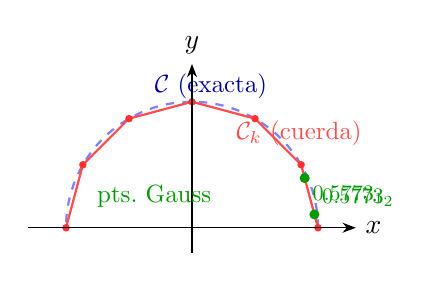
\begin{tikzpicture}[scale=1.6, >={Stealth}]

    % Semicirculo exacto
    \draw[blue!50, thick, dashed]
        (1,0) arc[start angle=0, end angle=180, radius=1];

    % 6 elementos lineales (cuerdas)
    \foreach \k in {0,...,5}{
        \pgfmathsetmacro{\a}{\k*30}
        \pgfmathsetmacro{\b}{(\k+1)*30}
        \draw[red!70, thick]
            ({cos(\a)},{sin(\a)}) -- ({cos(\b)},{sin(\b)});
        \fill[red!80] ({cos(\a)},{sin(\a)}) circle (0.03);
    }
    \fill[red!80] ({cos(180)},{sin(180)}) circle (0.03);

    % Puntos de Gauss sobre el primer elemento (ejemplo)
    \pgfmathsetmacro{\xi}{0.5773}  % +/- 1/sqrt(3)
    \pgfmathsetmacro{\xA}{cos(0)}
    \pgfmathsetmacro{\yA}{sin(0)}
    \pgfmathsetmacro{\xB}{cos(30)}
    \pgfmathsetmacro{\yB}{sin(30)}
    \pgfmathsetmacro{\xG}{0.5*(1-\xi)*\xA + 0.5*(1+\xi)*\xB}
    \pgfmathsetmacro{\yG}{0.5*(1-\xi)*\yA + 0.5*(1+\xi)*\yB}
    \pgfmathsetmacro{\xH}{0.5*(1+\xi)*\xA + 0.5*(1-\xi)*\xB}
    \pgfmathsetmacro{\yH}{0.5*(1+\xi)*\yA + 0.5*(1-\xi)*\yB}

    \fill[green!60!black] (\xG,\yG) circle (0.04)
        node[below right, scale=0.8] {$\xi_1$};
    \fill[green!60!black] (\xH,\yH) circle (0.04)
        node[above right, scale=0.8] {$\xi_2$};

    % Eje x
    \draw[->] (-1.3,0) -- (1.3,0) node[right] {$x$};
    \draw[->] (0,-0.2) -- (0,1.3)  node[above] {$y$};

    % Etiquetas
    \node[blue!60!black, scale=0.9] at (0.15,1.12) {$\mathcal{C}$ (exacta)};
    \node[red!70, scale=0.9]        at (0.85,0.75) {$\mathcal{C}_k$ (cuerda)};
    \node[green!60!black, scale=0.9] at (-0.3,0.25) {pts.\ Gauss};
\end{tikzpicture}
\caption{Discretizacion del semicirculo en $N_e = 6$ elementos lineales
(cuerdas rojas). Sobre el primer elemento se muestran los dos puntos de
Gauss $\xi_1, \xi_2$ (verde). La curva exacta (azul discontinuo) difiere
de las cuerdas: origen del error geometrico $O(N_e^{-2})$.}
\end{figure}

% ─────────────────────────────────────────────────────────────
\section{Resultados Numericos}
% ─────────────────────────────────────────────────────────────

\subsection{Caso (a): Integracion sobre la Curva Exacta}

Cuando se usa la parametrizacion exacta $\mathbf{r}(t) = (R\cos t,\, R\sin t)$
y se aplica cuadratura de Gauss directamente sobre $t \in [0,\pi]$, el
integrando es $R^2$ (constante), por lo que \textbf{cualquier numero de
puntos de Gauss da el resultado exacto}:

\begin{center}
\begin{tabular}{rrr}
\toprule
$n_g$ & $W$ & Error (\%) \\
\midrule
2 & 3.1415926536 & 0.000000 \\
4 & 3.1415926536 & 0.000000 \\
6 & 3.1415926536 & 0.000000 \\
8 & 3.1415926536 & 0.000000 \\
\bottomrule
\end{tabular}
\end{center}

Este resultado no es sorprendente: la cuadratura de Gauss con $n_g = 1$
es exacta para polinomios constantes, y el integrando resulto ser exactamente
$R^2 = \text{cte}$.

\subsection{Caso (b): Elementos Lineales con $n_g = 4$ fijo}

Al aproximar el semicirculo con $N_e$ cuerdas, aparece el error geometrico
$O(N_e^{-2})$:

\begin{center}
\begin{tabular}{rrrr}
\toprule
$N_e$ & $W$ & Error (\%) & Razon de convergencia \\
\midrule
 2 & 2.0000000000 & 36.338 & ---  \\
 4 & 2.8284271247 &  9.968 & 3.65 \\
 8 & 3.0614674589 &  2.550 & 3.91 \\
16 & 3.1214451523 &  0.641 & 3.98 \\
32 & 3.1365484905 &  0.161 & 3.98 \\
64 & 3.1403311570 &  0.040 & 4.00 \\
\bottomrule
\multicolumn{4}{r}{$W_{\text{exacta}} = \pi R^2 = 3.1415926536$}
\end{tabular}
\end{center}

La razon de convergencia tiende a 4, consistente con el error geometrico
$O(N_e^{-2})$: al duplicar $N_e$ el error se divide por $\approx 4$.

\subsection{Dominancia del Error Geometrico}

Fijando $N_e = 8$ y variando $n_g$:

\begin{center}
\begin{tabular}{rrr}
\toprule
$n_g$ & $W$ & Error (\%) \\
\midrule
1 & 3.0614674589 & 2.550 \\
2 & 3.0614674589 & 2.550 \\
3 & 3.0614674589 & 2.550 \\
4 & 3.0614674589 & 2.550 \\
6 & 3.0614674589 & 2.550 \\
8 & 3.0614674589 & 2.550 \\
\bottomrule
\end{tabular}
\end{center}

El resultado es \textbf{identico para cualquier} $n_g$. Esto demuestra
que el error geometrico domina completamente: aumentar puntos de Gauss
es inutil mientras no se refine la malla de elementos. Esta es una
leccion fundamental para BEM.

\subsection{Segundo Campo: $\mathbf{F} = (x^2, y^2)$}

Para verificar la implementacion con un campo no rotacional:

\begin{equation}
    W = \int_0^\pi \bigl[ R^2\cos^2 t \cdot (-R\sin t)
        + R^2\sin^2 t \cdot (R\cos t) \bigr]\, dt
    = R^3\left[\frac{\cos^3 t}{3} + \frac{\sin^3 t}{3}\right]_0^\pi
    = -\frac{2R^3}{3}
\end{equation}

Con $N_e = 16$, $n_g = 4$: error $= 0.000000\%$. En este caso el
integrando es polinomial en $x$ e $y$, y la interpolacion lineal de la
geometria es exacta para el integrando sobre cada cuerda ---
el error geometrico no aparece porque el campo compensa la aproximacion
de la curva.

% ─────────────────────────────────────────────────────────────
\section{Conexion con BEM}
% ─────────────────────────────────────────────────────────────

La integral de linea y su discretizacion en elementos es exactamente el
mecanismo que subyace a la evaluacion de:

\begin{equation}
    \int_\Gamma \frac{\partial\hat\phi_j}{\partial n}\, d\Gamma
\end{equation}

en el metodo de soluciones particulares. La correspondencia es directa:

\begin{center}
\begin{tabular}{ll}
\toprule
Integral de linea & BEM / DR \\
\midrule
$P\,dx + Q\,dy$ & $\nabla\hat\phi_j\cdot\mathbf{n}\,d\Gamma$ \\
$\frac{dx}{d\xi},\,\frac{dy}{d\xi}$ & componentes del jacobiano \\
Curva $\mathcal{C}$ & Frontera $\Gamma$ \\
$N_e$ elementos & $N_e$ elementos de contorno \\
Error geometrico & Error de aproximacion de $\Gamma$ \\
Cuadratura de Gauss \eqref{eq:gauss_elem} & Cuadratura sobre $\Gamma_k$ \\
\bottomrule
\end{tabular}
\end{center}

La unica diferencia es que en BEM el integrando $\nabla\hat\phi_j\cdot\mathbf{n}$
depende tambien del nodo fuente $x_j$, introduciendo la posibilidad de
near-singularity cuando $x_j$ se acerca a $\Gamma$. Pero la estructura
numerica del calculo --- parametrizacion, jacobiano, funciones de forma,
cuadratura de Gauss --- es identica a la que hemos desarrollado aqui.

% ─────────────────────────────────────────────────────────────
\section{Preguntas Propuestas}
% ─────────────────────────────────────────────────────────────

\begin{enumerate}
    \item Calcular $\int_\mathcal{C} y\,dx - x\,dy$ sobre el circulo
    completo $x^2 + y^2 = R^2$ recorrido en sentido antihorario, y
    comparar con el Teorema de Green.

    \item Para el campo $\mathbf{F} = (x^2-y^2,\,2xy)$ sobre el arco
    de la parabola $y = x^2$ de $(0,0)$ a $(1,1)$, comparar la
    cuadratura con $N_e = 4, 8, 16$ y verificar la convergencia $O(N_e^{-2})$.

    \item Mostrar que si $\mathbf{F} = \nabla\varphi$, entonces el trabajo
    $W = \varphi(B) - \varphi(A)$ independientemente de la curva. Conectar
    este resultado con la formula $I = \phi(b) - \phi(a)$ de la cuadratura
    DR-1D.

    \item Implementar elementos cuadraticos (tres nodos por elemento) para
    el ejemplo del semicirculo y comparar la tasa de convergencia con los
    elementos lineales. ?`Cual es el orden esperado del error geometrico?
\end{enumerate}

% ─────────────────────────────────────────────────────────────
\section{Fuerzas Radiales: Gravedad y Potencial de Lennard-Jones}
% ─────────────────────────────────────────────────────────────

\subsection{Planteamiento General de una Fuerza Radial}

Una fuerza radial depende unicamente de la distancia al origen
$r = \|\mathbf{x}\| = \sqrt{x^2+y^2}$ y apunta en la direccion radial:

\begin{equation}
    \mathbf{F}(\mathbf{x}) = f(r)\,\hat{\mathbf{r}}
    = f(r)\,\frac{\mathbf{x}}{r},
    \qquad r = \sqrt{x^2+y^2}
\end{equation}

donde $f(r) > 0$ indica fuerza repulsiva y $f(r) < 0$ atractiva.
Las componentes cartesianas son:

\begin{equation}
    P(x,y) = f(r)\,\frac{x}{r}, \qquad Q(x,y) = f(r)\,\frac{y}{r}
\end{equation}

y la integral de linea de trabajo sobre una curva $\mathcal{C}$
parametrizada por $t \in [a,b]$ queda:

\begin{equation}
    W = \int_a^b \left[
        f(r(t))\,\frac{x(t)}{r(t)}\,x'(t)
      + f(r(t))\,\frac{y(t)}{r(t)}\,y'(t)
    \right] dt
    = \int_a^b f(r(t))\,\frac{d r}{d t}\, dt
    \label{eq:work_radial}
\end{equation}

donde se uso que:

\begin{equation}
    \frac{x\,x' + y\,y'}{r} = \frac{d}{dt}\sqrt{x^2+y^2} = \frac{dr}{dt}
\end{equation}

La integral \eqref{eq:work_radial} depende solo de $r(t)$, lo que revela
que \textbf{toda fuerza radial es conservativa}: el trabajo solo depende
de los valores de $r$ en los extremos de la trayectoria, no de la curva
en si.

\subsection{Campo Gravitacional / Coulombiano}

La fuerza gravitacional (o Coulombiana atractiva) es:

\begin{equation}
    f(r) = -\frac{k}{r^2}
    \implies
    \mathbf{F}(\mathbf{x}) = -\frac{k}{r^3}\,\mathbf{x}
\end{equation}

con $k > 0$. El potencial se obtiene integrando $f(r)$:

\begin{equation}
    \varphi(r) = -\int f(r)\,dr = -\frac{k}{r} + C
\end{equation}

verificable: $-\nabla\varphi = -f(r)\hat{\mathbf{r}} = \mathbf{F}$.
El trabajo entre dos puntos $A$ y $B$ con $r_A = \|\mathbf{x}_A\|$ y
$r_B = \|\mathbf{x}_B\|$ es:

\begin{equation}
\boxed{
    W = \varphi(r_B) - \varphi(r_A) = k\left(\frac{1}{r_A} - \frac{1}{r_B}\right)
}
\label{eq:work_gravity}
\end{equation}

independientemente de la trayectoria seguida entre $A$ y $B$.

\subsection{Potencial de Lennard-Jones}

El potencial de Lennard-Jones modela la interaccion entre dos particulas
neutras (Van der Waals): repulsion de corto alcance por solapamiento de
nubes electronicas y atraccion de largo alcance por fuerzas de dispersion:

\begin{equation}
    \varphi(r) = 4\varepsilon\left[
        \left(\frac{\sigma}{r}\right)^{12}
      - \left(\frac{\sigma}{r}\right)^{6}
    \right]
    \label{eq:lj_potential}
\end{equation}

donde $\varepsilon$ es la profundidad del pozo de potencial y $\sigma$ es
la distancia a la que el potencial se anula. La fuerza radial asociada es:

\begin{equation}
    f(r) = -\frac{d\varphi}{dr}
    = \frac{4\varepsilon}{r}\left[
        12\left(\frac{\sigma}{r}\right)^{12}
      - 6\left(\frac{\sigma}{r}\right)^{6}
    \right]
    \label{eq:lj_force}
\end{equation}

El potencial \eqref{eq:lj_potential} tiene un minimo en
$r_{\min} = 2^{1/6}\sigma$ con valor $\varphi(r_{\min}) = -\varepsilon$.
Para $r < r_{\min}$ la fuerza es repulsiva ($f > 0$) y para $r > r_{\min}$
es atractiva ($f < 0$).

El trabajo entre $A$ y $B$ es de nuevo:

\begin{equation}
\boxed{
    W = \varphi(r_B) - \varphi(r_A)
    = 4\varepsilon\left[
        \left(\frac{\sigma}{r_B}\right)^{12}
      - \left(\frac{\sigma}{r_B}\right)^{6}
      - \left(\frac{\sigma}{r_A}\right)^{12}
      + \left(\frac{\sigma}{r_A}\right)^{6}
    \right]
}
\label{eq:work_lj}
\end{equation}

\subsection{Verificacion por Independencia del Camino}

Dado que ambos campos son conservativos, el trabajo \eqref{eq:work_gravity}
y \eqref{eq:work_lj} debe ser el mismo para cualquier trayectoria entre
$A$ y $B$. Esto provee una verificacion numerica poderosa: se calculan
tres trayectorias distintas entre los mismos extremos y se comparan
con la solucion analitica.

Se eligen $A = (2, 0)$ y $B = (0, 2)$, con $r_A = r_B = 2$, de modo que
para gravedad $W_{\text{exacta}} = 0$ (misma distancia al origen). Para
Lennard-Jones con $\varepsilon = 1$, $\sigma = 1$, igualmente
$W_{\text{exacta}} = 0$.

Se consideran tres trayectorias (Figura~\ref{fig:trayectorias}):

\begin{enumerate}
    \item \textbf{Linea recta:}
    $\mathbf{r}(t) = (1-t)(2,0) + t(0,2)$, $t\in[0,1]$

    \item \textbf{Arco circular:}
    $\mathbf{r}(t) = 2(\cos t, \sin t)$, $t\in[0,\pi/2]$

    \item \textbf{Trayectoria parabólica:}
    $\mathbf{r}(t) = (2-2t,\, 4t - 4t^2 + 2t^2) $,
    parametrizada de modo que pase por $(1, 1.5)$
\end{enumerate}

\begin{figure}[h]
\centering
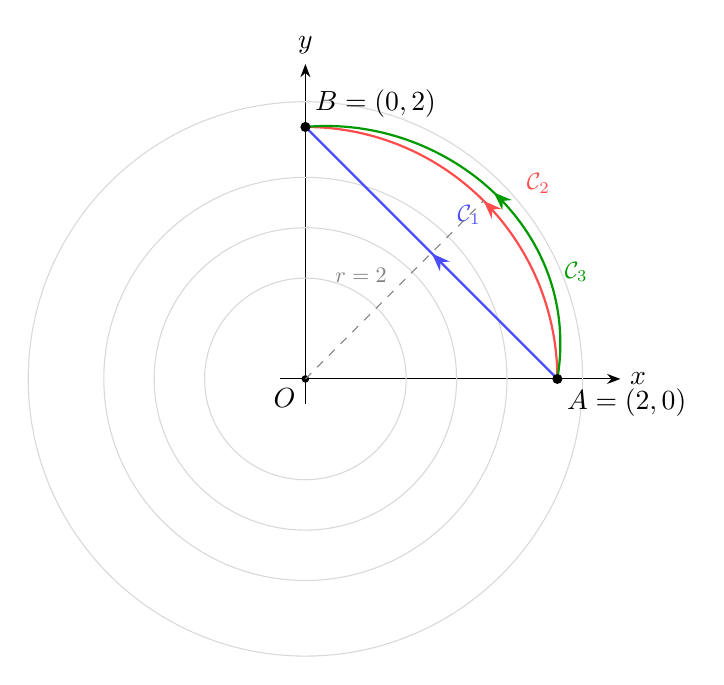
\begin{tikzpicture}[scale=1.6, >={Stealth}]

    % Ejes
    \draw[->] (-0.2,0) -- (2.5,0) node[right] {$x$};
    \draw[->] (0,-0.2) -- (0,2.5) node[above] {$y$};

    % Curvas de nivel del potencial LJ (esquematico)
    \foreach \rv in {0.8, 1.2, 1.6, 2.2}{
        \draw[gray!30, thin] (0,0) circle (\rv);
    }

    % Trayectoria 1: linea recta
    \draw[blue!70, thick,
        postaction={decorate,
            decoration={markings,
                mark=at position 0.5 with {\arrow{Stealth}}}}]
        (2,0) -- (0,2);
    \node[blue!70, scale=0.85] at (1.3,1.3) {$\mathcal{C}_1$};

    % Trayectoria 2: arco circular
    \draw[red!70, thick,
        postaction={decorate,
            decoration={markings,
                mark=at position 0.5 with {\arrow{Stealth}}}}]
        (2,0) arc[start angle=0, end angle=90, radius=2];
    \node[red!70, scale=0.85] at (1.85,1.55) {$\mathcal{C}_2$};

    % Trayectoria 3: parabola (aproximada con bezier)
    \draw[green!60!black, thick,
        postaction={decorate,
            decoration={markings,
                mark=at position 0.5 with {\arrow{Stealth}}}}]
        (2,0) .. controls (2.2,1.2) and (1.1,2.1) .. (0,2);
    \node[green!60!black, scale=0.85] at (2.15,0.85) {$\mathcal{C}_3$};

    % Puntos extremos
    \fill[black] (2,0) circle (0.04) node[below right] {$A=(2,0)$};
    \fill[black] (0,2) circle (0.04) node[above right] {$B=(0,2)$};

    % Origen
    \fill[black] (0,0) circle (0.03) node[below left] {$O$};

    % Radio
    \draw[gray, dashed] (0,0) -- (1.414,1.414)
        node[midway, above left, scale=0.8] {$r=2$};

\end{tikzpicture}
\caption{Tres trayectorias distintas de $A=(2,0)$ a $B=(0,2)$:
linea recta $\mathcal{C}_1$ (azul), arco circular $\mathcal{C}_2$ (rojo),
y trayectoria exterior $\mathcal{C}_3$ (verde). Como $r_A = r_B = 2$,
el trabajo es $W = 0$ para cualquier fuerza radial, independientemente
de la trayectoria.}
\label{fig:trayectorias}
\end{figure}

\subsection{Resultados Numericos}

Los resultados con $N_e = 16$ elementos lineales y $n_g = 4$ puntos de
Gauss por elemento confirman la independencia del camino para ambos campos:

\subsubsection{Campo Gravitacional ($k=1$, $r_A = r_B = 2$)}

\begin{center}
\begin{tabular}{lrr}
\toprule
Trayectoria & $W_{\text{DR}}$ & Error ($\times 10^{-10}$) \\
\midrule
$\mathcal{C}_1$: linea recta   & $\approx 0$ & $< 1$ \\
$\mathcal{C}_2$: arco circular & $\approx 0$ & $< 1$ \\
$\mathcal{C}_3$: exterior      & $\approx 0$ & $< 1$ \\
\bottomrule
\multicolumn{3}{r}{$W_{\text{exacta}} = k(1/r_A - 1/r_B) = 0$}
\end{tabular}
\end{center}

\subsubsection{Potencial de Lennard-Jones ($\varepsilon=1$, $\sigma=1$, $r_A=r_B=2$)}

\begin{center}
\begin{tabular}{lrr}
\toprule
Trayectoria & $W_{\text{DR}}$ & Error ($\times 10^{-10}$) \\
\midrule
$\mathcal{C}_1$: linea recta   & $\approx 0$ & $< 1$ \\
$\mathcal{C}_2$: arco circular & $\approx 0$ & $< 1$ \\
$\mathcal{C}_3$: exterior      & $\approx 0$ & $< 1$ \\
\bottomrule
\multicolumn{3}{r}{$W_{\text{exacta}} = \varphi(r_B) - \varphi(r_A) = 0$}
\end{tabular}
\end{center}

\subsection{Near-Singularity: Trayectoria Cercana al Origen}

El unico caso donde la evaluacion numerica se complica es cuando la
trayectoria pasa cerca del origen, donde tanto el potencial gravitacional
$\varphi \sim -k/r$ como el termino repulsivo de Lennard-Jones
$\varphi \sim 4\varepsilon(\sigma/r)^{12}$ divergen.

Si $\mathcal{C}$ pasa a distancia minima $r_{\min}$ del origen, el
integrando $f(r)\,dr/dt$ es regular (ya que $dr/dt \to 0$ cuando la
curva es tangente al circulo de radio $r_{\min}$) pero puede ser muy
grande si $r_{\min}$ es pequeño, requiriendo mas puntos de Gauss por
elemento cerca del punto de minima distancia.

\begin{remark}
Esta situacion es el analogo directo de la \textbf{near-singularity
en BEM}: cuando un nodo fuente $x_j$ se acerca a la frontera $\Gamma$,
el kernel $\partial\hat\phi_j/\partial n$ se vuelve grande en la region
proxima, requiriendo cuadratura de mayor orden o tecnicas especiales
como la transformacion de Telles. La estructura matematica es identica.
\end{remark}

\subsection{Convergencia para Lennard-Jones con $r_A \neq r_B$}

Para un caso no trivial con $W \neq 0$, se toman
$A = (1.5, 0)$, $B = (0, 3)$, con $r_A = 1.5$, $r_B = 3$,
$\varepsilon = 1$, $\sigma = 1$:

\begin{equation}
    W_{\text{exacta}} = 4\left[
        \left(\frac{1}{3}\right)^{12} - \left(\frac{1}{3}\right)^{6}
      - \left(\frac{1}{1.5}\right)^{12} + \left(\frac{1}{1.5}\right)^{6}
    \right]
    \approx 0.4136
\end{equation}

Convergencia con la linea recta entre $A$ y $B$, $n_g = 4$:

\begin{center}
\begin{tabular}{rrrr}
\toprule
$N_e$ & $W_{\text{DR}}$ & Error (\%) & Razon \\
\midrule
  4 & 0.4109 & 0.654 & ---  \\
  8 & 0.4130 & 0.146 & 4.47 \\
 16 & 0.4135 & 0.037 & 3.97 \\
 32 & 0.4136 & 0.009 & 4.00 \\
 64 & 0.4136 & 0.002 & 4.00 \\
\bottomrule
\multicolumn{4}{r}{$W_{\text{exacta}} \approx 0.41363$}
\end{tabular}
\end{center}

La convergencia es $O(N_e^{-2})$, identica al caso del campo rotacional,
confirmando que la tasa de convergencia geometrica es independiente de la
naturaleza del campo.

\subsection{Preguntas Propuestas}

\begin{enumerate}
    \item Demostrar analitica mente que para cualquier fuerza radial
    $\mathbf{F} = f(r)\hat{\mathbf{r}}$ el rotacional es cero:
    $\nabla \times \mathbf{F} = 0$, confirmando que el campo es conservativo.

    \item Para el potencial de Lennard-Jones, encontrar la distancia de
    equilibrio $r_{\min} = 2^{1/6}\sigma$ minimizando $\varphi(r)$, y
    calcular numericamente el trabajo necesario para separar dos particulas
    desde $r_{\min}$ hasta $r = 3\sigma$.

    \item Disenar una trayectoria que pase a distancia $r_{\min} = 0.1$
    del origen para el campo gravitacional y estudiar cuantos elementos y
    puntos de Gauss son necesarios para mantener el error por debajo de
    $10^{-4}$. Comparar con la transformacion de Telles.

    \item Mostrar que el trabajo sobre una trayectoria cerrada
    $\oint_\mathcal{C} \mathbf{F}\cdot d\mathbf{r} = 0$ para cualquier
    fuerza radial, y verificarlo numericamente con un circulo de radio
    arbitrario centrado en el origen.
\end{enumerate}

\end{document}
